\scanpage{64}
\diagram{
\begin{tikzcd}[column sep=large,row sep=large]
e\arrow[r]&\begin{gathered}SO(2n)\\\text{centre }\mu_2\end{gathered}\arrow[r,dash]&O(2n)\arrow[r]\arrow[dr,dashed,"\text{dét}"']&\mathbf Z/2\mathbf Z\arrow[r,dash]\arrow[d]&e\\
&\underbrace{\hspace{4cm}}_{\text{centre }\mu_2}&&\unsure{\mathbf G_m}\arrow[ul,phantom,"{\begin{gathered}\text{produit}\\\text{semi-direct}\end{gathered}}"]&
\end{tikzcd}
}

\diagram{
\begin{tikzcd}[column sep=large,row sep=large]
e\arrow[r]&\begin{gathered}SO(2n+1)\\\text{centre }\{e\}\end{gathered}\arrow[r]&O(2n+1)\arrow[r]\arrow[dr,dashed,"\text{dét}"']&\mu_2\arrow[r,dash]\arrow[d]&e\\
&\underbrace{\hspace{4cm}}_{\text{centre }\mu_2}&&G_m\arrow[ul,phantom,"{\begin{gathered}\text{prod.}\\\text{semi-}\\\text{direct}\end{gathered}}"]&
\end{tikzcd}
}

Pour tout entier $m$, on a
\diagram{
\begin{tikzcd}[column sep=large,row sep=large]
e\arrow[r,dash]&\mu_2\arrow[r]&\operatorname{Pin}(m)\arrow[r]&O(m)\arrow[r,dash]&e\\
e\arrow[r,dash]&\mu_2\arrow[u,equal]\arrow[r,dash]&\operatorname{Spin}(m)\arrow[u,"{\deleted{\unsure{Spin(m)}}}"']\arrow[r,dash]&SO(m)\arrow[u]\arrow[r,dash]&e
\end{tikzcd}
}

\margin{$\deleted{\unsure{(\xi)}}\ \unsure{\xi'}$\quad En car, $2$
\[
(x,y)\longrightarrow(\unsure{\lambda}x+\unsure{v|u}(y),y)
\]
\figure{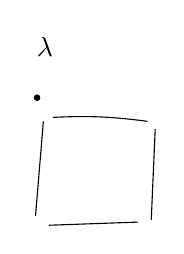
\begin{tikzpicture}[x=1cm,y=1cm]
\node at (0,2.25) {$\lambda$};
\fill (-0.1,1.6) circle (1.2pt);
\draw (0.1,1.35) to[bend left=5] (1.3,1.3);
\draw (-0.02,1.3)--(-0.12,0.1);
\draw (1.4,1.2)--(1.35,0.05);
\draw (0.05,-0.02)--(1.18,0.02);
\end{tikzpicture}}
\[
(\lambda(x)+v(y))^2+Q(y)
\]
\[
\lambda^2x^2+v(y)^2=x^2
\]
\[
v(y)^2=0
\]
\[
\lambda^2=1
\]
\[
v(y)^2=
\]
\[
\uline{\lambda^2=1}\qquad\mu_2
\]
\diagram{\[
\left(\begin{array}{ccccc}
\mu_2&\alpha_2&\alpha_2&\mathbin{-}\mathbin{-}&\alpha_2\\[1cm]
&&&&
\end{array}\right)
\]}

$\deleted{\unsure{x\longmapsto\lambda}}$
\[
(\xi,y)\longrightarrow(\lambda\xi+u(y),y)
\]
\[
\lambda^2=1\qquad u(y)^2=0
\]
\[
\lambda'\lambda\xi+\lambda'u(y)+u'(y)
\]
\[
(\lambda',u')(\lambda,u)=(\lambda'\lambda,\lambda'u+u')
\]
\[
\mu_2.
\]
}
\margin{63}
